\chapter{Advanced Topics}

This chapter explains how you can customize the \NanoXML{} parser setup.
Unlike \ltext{NanoXML 1}, \ltext{NanoXML/Java 2} is designed as a framework: it is composed of many different components which you can plug together.
It's possible to change the reader, the builder, the validator and even the parser.

\ltext{NanoXML/Java} comes with one set of components.
Except for \ltext{NanoXML/Lite}, every branch offers its own set of components customized for a certain purpose.
\ltext{NanoXML/SAX} offers components for using \NanoXML{} as a parser for the \ltext{SAX} framework.

The following figure gives a short representation of the major components.

\begin{figure}[ht]
\begin{center}
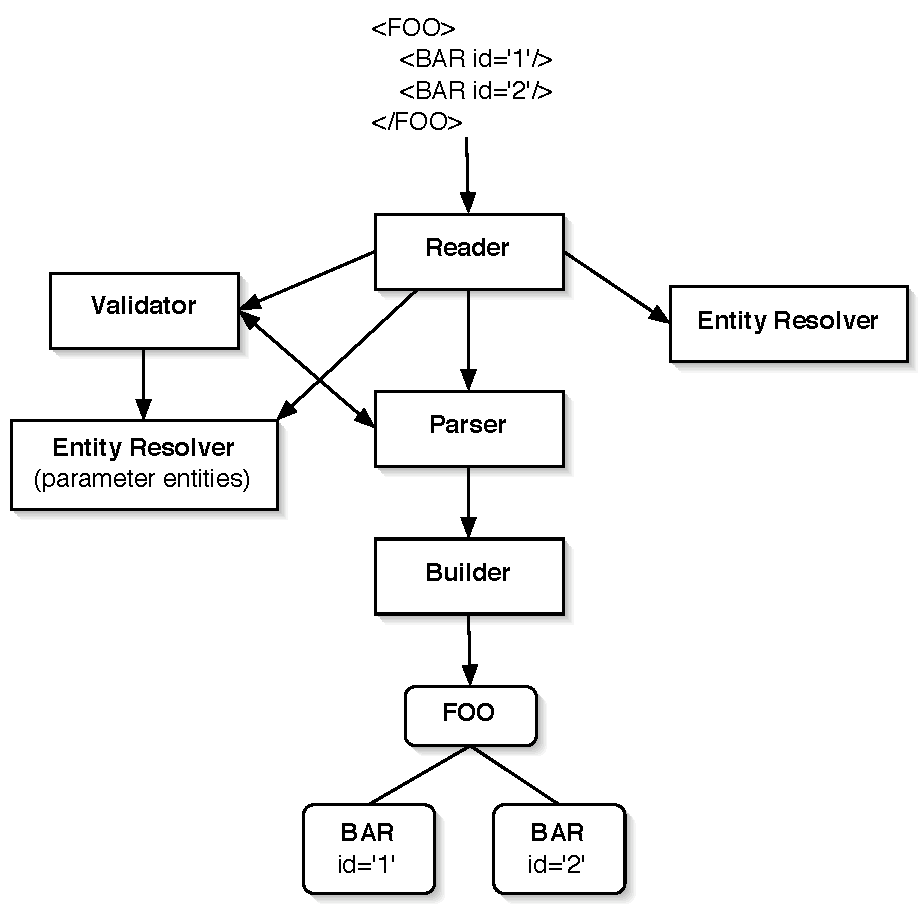
\includegraphics[width=8cm]{structure.pdf}
\end{center}
\caption{Design of NanoXML/Java}
\end{figure}

The \emph{reader} retrieves data from a Java input stream and provides character data to the other components.

The \emph{parser} converts the character data it retrieves from the reader to \XML{} events which it sends to the builder.

The \emph{validator} parses a \ltext{DTD} and validates the \XML{} data.
The current validator does only the minimum necessary for a non-validating parser.

The \emph{entity resolvers} converts entity references (\&\ldots;) and parameter entity references (\%\ldots;) to character data.
The resolver uses the reader to access external entities.

The \emph{builder} interpretes \XML{} events coming from the parser and builds a tree of \XML{} elements.
The standard builder creates a tree of \classname{IXMLElement}.
You can provide your own builder to create a custom tree or if you are interested in the \XML{} events themselves, \acronym{e.g.} to use \XML{} streaming.


\section{The \NanoXML{} Reader}

The reader retrieves data from some source and feeds it to the other components.

The reader is basically a stack of push-back readers.
Every time a new data stream becomes active, the current reader is pushed on a stack.
When the current reader has no more data left, the parent reader is popped from the stack.

If you want to implement public IDs using \acronym{e.g.} a catalog file similar to SGML, you could implement a reader by overriding the method \methodname{openStream} of \classname{StdXMLReader}:

\begin{example}
\xkeyword{public class} MyReader
~~\xkeyword{extends} StdXMLReader
\{
~~\xkeyword{private} Properties publicIDs;
~
~~\xkeyword{public} MyReader(Properties publicIDs)
~~\{
~~~~\xkeyword{this}.publicIDs = publicIDs;
~~\}
~
~~\xkeyword{public} Reader openStream(String publicID,
~~~~~~~~~~~~~~~~~~~~~~~~~~~String systemID)
~~~~\xkeyword{throws} MalformedURLException,
~~~~~~~~~~~FileNotFoundException,
~~~~~~~~~~~IOException
~~\{
~~~~\xkeyword{if} (publicID != \xkeyword{null}) \{
~~~~~~systemID = publicIDs.getProperty(publicID, systemID);
~~~~\}
~~~~\xkeyword{return super}.openStream(publicID, systemID);
~~\}
\}
\end{example}

In this example, you have to provide a properties object which maps public IDs to system IDs.


\section{The \NanoXML{} Parser}

The parser analyzes the character stream it retrieves from the reader and sends \XML{} events to the builder.
It uses a validator to validate the data and an entity resolver to resolve general entities.
You rarely need to create a custom parser.
If you need to, you have to implement \classname{IXMLParser}.


\section{The \NanoXML{} Validator}

The validator parses the \ltext{DTD} and checks the \XML{} data.
\ltext{NanoXML 2.0} uses a \classname{NonValidator} implementation that only performs the minimum necessary for a non-validating parser.

As a \ltext{DTD} is very vague, you can implement your own validator to perform a more fine-grained check of the \XML{} data.
The easiest way to create your own validator is to create a subclass of \classname{ValidatorPlugin}.

The following example shows how to implement a validator.
It checks that every attribute named ``id'' starts with three capital letters.

\begin{example}
\xkeyword{public class} MyValidator
~~\xkeyword{extends} ValidatorPlugin
\{
~~\xkeyword{public void} attributeAdded(String key,
~~~~~~~~~~~~~~~~~~~~~~~~~~~~~String value,
~~~~~~~~~~~~~~~~~~~~~~~~~~~~~String systemID,
~~~~~~~~~~~~~~~~~~~~~~~~~~~~~\xkeyword{int} lineNr)
~~\{
~~~~\xkeyword{boolean} valid = true;
~~~~\xkeyword{if} (key.equals("id")) \{
~~~~~~\xkeyword{if} (value.length() < 3) \{
~~~~~~~~valid = \xkeyword{false};
~~~~~~\} \xkeyword{else} \{
~~~~~~~~\xkeyword{for} (\xkeyword{int} i = 0; i < 3; i++) \{
~~~~~~~~~~\xkeyword{char} ch = value.charAt(i);
~~~~~~~~~~\xkeyword{if} ((ch < 'A') || (ch > 'Z')) \{
~~~~~~~~~~~~valid = \xkeyword{false};
~~~~~~~~~~\}
~~~~~~~~\}
~~~~~~\}
~~~~\}
~~~~\xkeyword{if} (valid) \{
~~~~~~\xkeyword{super}.attributeAdded(key, value, systemID, lineNr);
~~~~\} \xkeyword{else} \{
~~~~~~\xkeyword{this}.attributeWithInvalidValue(systemID, lineNr, \xkeyword{null}, key, value);
~~~~\}
~~\}
\}
\end{example}

To register the validator to a parser, use the following code:

\begin{example}
IXMLParser parser \ldots
\ldots
IXMLValidator val1 = parser.getValidator();
MyValidator val2 = \xkeyword{new} MyValidator();
val2.setDelegate(val1);
parser.setValidator(val2);
\end{example}


\section{The \NanoXML{} Entity Resolvers}

The entity resolver converts entity references to \XML{} data.
If you want \acronym{e.g.} to retrieve entity values from a database, you have to create your own resolver.

Entity resolvers have to implement \classname{IXMLEntityResolver}.
Usually, you only have to make a subclass of \classname{XMLEntityResolver} and implement the method \methodname{getEntity} or \methodname{openExternalEntity}.

Entities can be used in the \XML{} data and in the \ltext{DTD}.
As these entities are independent of each other, there are two entity resolvers.


\subsection{Standard Entities}

The resolver for standard entities has to be registered to the parser by calling \methodname{setResolver}.
The following example registers a resolver that forces the entity ``\&foo;'' to be resolved to ``bar'':

\begin{example}
\xkeyword{import} net.n3.nanoxml.*;
\xkeyword{import} java.io.*;
~
\xkeyword{class} MyResolver
~~\xkeyword{extends} XMLEntityResolver
\{
~~\xkeyword{public} Reader getEntity(IXMLReader xmlReader,
~~~~~~~~~~~~~~~~~~~~~~~~~~String name)
~~~~\xkeyword{throws} XMLParseException
~~\{
~~~~\xkeyword{if} (name.equals("foo")) \{
~~~~~~\xkeyword{return new} StringReader("bar");
~~~~\} \xkeyword{else} \{
~~~~~~\xkeyword{return super}.getEntity(xmlReader, name);
~~~~\}
~~\}
\}
~
\xkeyword{public class} Demo
\{
~~\xkeyword{public static void} main(String[] args)
~~~~\xkeyword{throws} Exception
~~\{
~~~~IXMLParser parser = XMLParserFactory.createDefaultXMLParser();
~~~~parser.setResolver(new MyResolver());
~~~~IXMLReader reader = StdXMLReader.fileReader("test.xml");
~~~~parser.setReader(reader);
~~~~IXMLElement xml = (IXMLElement) parser.parse();
~~~~XMLWriter writer = new XMLWriter(System.out);
~~~~writer.write(xml);
~~\}
\}
\end{example}


\subsection{Parameter Entities}

The resolver for parameter entities has to be registered to the validator by calling \methodname{setParameterEntityResolver}.
The following example show a custom version of the \classname{Demo} class that registers \methodname{MyResolver} as a parameter entity resolver.

\begin{example}
\xkeyword{public class} Demo
\{
~~\xkeyword{public static void} main(String[] args)
~~~~\xkeyword{throws} Exception
~~\{
~~~~IXMLParser parser = XMLParserFactory.createDefaultXMLParser();
~~~~IXMLValidator validator = parser.getValidator();
~~~~validator.setParameterEntityResolver(new MyResolver());
~~~~IXMLReader reader = StdXMLReader.fileReader("test.xml");
~~~~parser.setReader(reader);
~~~~IXMLElement xml = (IXMLElement) parser.parse();
~~~~XMLWriter writer = new XMLWriter(System.out);
~~~~writer.write(xml);
~~\}
\}
\end{example}


\section{The \NanoXML{} Builder}

The builder interpretes \XML{} events coming from the parser and builds a tree of \ltext{Java} objects.
When the parsing is done, the builder hands over its result to the parser.

As explained in chapter 3, the builder can also be used to read \XML{} data while it's being streamed.
This feature is useful if you don't want to wait until all the data has been read before processing the information.

As an example, we have the following XML structure (document.dtd):

\begin{example}
$<$!ELEMENT Chapter (Paragraph*)$>$
$<$!ATTLIST Chapter
~~~~~~~~title~CDATA~\#REQUIRED
~~~~~~~~id~~~~CDATA~\#REQUIRED$>$
$<$!ELEMENT Paragraph (\#PCDATA)$>$
$<$!ATTLIST Paragraph
~~~~~~~~align~(left|center|right)~"left"$>$
\end{example}

The elements are put in the \ltext{Java} classes \classname{Chapter} and \classname{Paragraph} which, for convenience, extend the following base class:

\begin{example}
\xkeyword{public class} DocumentElement
\{
~~\xkeyword{protected} Properties attrs;
~~\xkeyword{protected} Vector children;
~
~~\xkeyword{public} DocumentElement()
~~\{
~~~~\xkeyword{this}.attrs = \xkeyword{new} Properties();
~~~~\xkeyword{this}.children = \xkeyword{new} Vector();
~~\}
~
~~\xkeyword{public void} setAttribute(String attrName,
~~~~~~~~~~~~~~~~~~~~~~~~~~~String value)
~~\{
~~~~\xkeyword{this}.attrs.put(attrName, value);
~~\}
~
~~\xkeyword{public void} addChild(DocumentElement elt)
~~\{
~~~~\xkeyword{this}.children.addElement(elt);
~~\}
\}
\end{example}

This base class simply makes it easy for our builder to set attributes and to add children to an element.

The \classname{Chapter} and \classname{Paragraph} classes extend this base class to give more practical access to their attributes and children:

\begin{example}
\xkeyword{public class} Chapter
~~\xkeyword{extends} DocumentElement
\{
~~\xkeyword{public} String getTitle()
~~\{
~~~~\xkeyword{return this}.attrs.getProperty("title");
~~\}
~
~~\xkeyword{public} String getID()
~~\{
~~~~\xkeyword{return this}.attrs.getProperty("id");
~~\}
~
~~\xkeyword{public} Enumeration getParagraphs()
~~\{
~~~~\xkeyword{return this}.children.elements();
~~\}
\}
~
\xkeyword{public class} Paragraph
~~\xkeyword{extends} DocumentElement
\{
~~\xkeyword{public static final int} LEFT = 0;
~~\xkeyword{public static final int} CENTER = 1;
~~\xkeyword{public static final int} RIGHT = 2;
~
~~\xkeyword{private static} Hashtable alignments;
~
~~\xkeyword{static}
~~\{
~~~~alignments = \xkeyword{new} Hashtable();
~~~~alignments.put("left", \xkeyword{new} Integer(LEFT));
~~~~alignments.put("center", \xkeyword{new} Integer(CENTER));
~~~~alignments.put("right", \xkeyword{new} Integer(RIGHT));
~~\}
~
~~\xkeyword{public} String getContent()
~~\{
~~~~\xkeyword{return this}.attrs.getProperty("\#PCDATA");
~~\}
~
~~\xkeyword{public int} getAlignment()
~~\{
~~~~String str = \xkeyword{this}.attrs.getProperty("align");
~~~~Integer align = alignments.get(str);
~~~~\xkeyword{return} align.intValue();
~~\}
\}
\end{example}

The builder creates the data structure based on the \XML{} events it receives from the parser.
Because both \classname{Chapter} and \classname{Paragraph} extend \classname{DocumentElement}, the builder is fairly simple.

\begin{example}
\xkeyword{import} net.n3.nanoxml.*;
\xkeyword{import} java.util.*;
\xkeyword{import} java.io.*;
~
\xkeyword{public class} DocumentBuilder
~~\xkeyword{implements} IXMLBuilder
\{
~~\xkeyword{private static} Hashtable classes;
~~\xkeyword{private} Stack elements;
~~\xkeyword{private} DocumentElement topElement;
~
~~\xkeyword{static}
~~\{
~~~~classes = \xkeyword{new} Hashtable();
~~~~classes.put("Chapter", Chapter.\xkeyword{class});
~~~~classes.put("Paragraph", Paragraph.\xkeyword{class});
~~\}
~
~~\xkeyword{public void} startBuilding(String systemID,
~~~~~~~~~~~~~~~~~~~~~~~~~~~~\xkeyword{int} lineNr)
~~\{
~~~~\xkeyword{this}.elements = \xkeyword{new} Stack();
~~~~\xkeyword{this}.topElement = \xkeyword{null};
~~\}
~
~~\xkeyword{public void} newProcessingInstruction(String target,
~~~~~~~~~~~~~~~~~~~~~~~~~~~~~~~~~~~~~~~Reader reader)
~~\{
~~~~// nothing to do
~~\}
~
~~\xkeyword{public void} startElement(String name,
~~~~~~~~~~~~~~~~~~~~~~~~~~~String nsPrefix,
~~~~~~~~~~~~~~~~~~~~~~~~~~~String nsSystemID,
~~~~~~~~~~~~~~~~~~~~~~~~~~~String systemID,
~~~~~~~~~~~~~~~~~~~~~~~~~~~\xkeyword{int} lineNr)
~~\{
~~~~DocumentElement elt = \xkeyword{null};
~~~~\xkeyword{try} \{
~~~~~~Class cls = (Class) classes.get(name);
~~~~~~elt = (DocumentElement) cls.newInstance();
~~~~\} \xkeyword{catch} (Exception e) \{
~~~~~~// ignore the exception
~~~~\}
~~~~\xkeyword{this}.elements.push(elt);
~~~~\xkeyword{if} (\xkeyword{this}.topElement == \xkeyword{null}) \{
~~~~~~\xkeyword{this}.topElement = elt;
~~~~\}
~~\}
~
~~\xkeyword{public void} endElement(String name,
~~~~~~~~~~~~~~~~~~~~~~~~~String nsPrefix,
~~~~~~~~~~~~~~~~~~~~~~~~~String nsSystemID)
~~\{
~~~~DocumentElement child = (DocumentElement) \xkeyword{this}.elements.pop();
~~~~\xkeyword{if} (! \xkeyword{this}.elements.isEmpty()) \{
~~~~~~DocumentElement parent = (DocumentElement) \xkeyword{this}.elements.peek();
~~~~~~parent.addChild(child);
~~~~\}
~~\}
~
~~\xkeyword{public void} addAttribute(String key,
~~~~~~~~~~~~~~~~~~~~~~~~~~~String nsPrefix,
~~~~~~~~~~~~~~~~~~~~~~~~~~~String nsSystemID,
~~~~~~~~~~~~~~~~~~~~~~~~~~~String value,
~~~~~~~~~~~~~~~~~~~~~~~~~~~String type)
~~\{
~~~~DocumentElement child = (DocumentElement) \xkeyword{this}.elements.peek();
~~~~child.setAttribute(key, value);
~~\}
~
~~\xkeyword{public void} elementAttributesProcessed(String name,
~~~~~~~~~~~~~~~~~~~~~~~~~~~~~~~~~~~~~~~~~String nsPrefix,
~~~~~~~~~~~~~~~~~~~~~~~~~~~~~~~~~~~~~~~~~String nsSystemID)
~~\{
~~~~// nothing to do
~~\}
~
~~\xkeyword{public void} addPCData(Reader reader,
~~~~~~~~~~~~~~~~~~~~~~~~String systemID,
~~~~~~~~~~~~~~~~~~~~~~~~\xkeyword{int} lineNr)
~~~~\xkeyword{throws} IOException
~~\{
~~~~StringBuffer str = \xkeyword{new} StringBuffer(1024);
~~~~\xkeyword{char}[] buf = \xkeyword{new char}[bufSize];
~~~~\xkeyword{for} (;;) \{
~~~~~~\xkeyword{int} size = reader.read(buf);
~~~~~~\xkeyword{if} (size < 0) \{
~~~~~~~~\xkeyword{break};
~~~~~~\}
~~~~~~str.append(buf, 0, size);
~~~~\}
~~~~\xkeyword{this}.addAttribute("\#PCDATA", \xkeyword{null}, \xkeyword{null}, str.toString(), "CDATA");
~~\}
~
~~\xkeyword{public} Object getResult()
~~\{
~~~~\xkeyword{return} topElement;
~~\}
\}
\end{example}

Note that, for simplicity, error and exception handling is not present in this example.
The builder holds a stack of the current elements it builds.
Character data is read from a reader.
The method \methodname{addPCData} reads this data in blocks of 1K.

Finally, this application sets up the \NanoXML{} parser and converts an \XML{} document to \ltext{HTML} which it dumps on the standard output:

\begin{example}
\xkeyword{import} java.util.*;
\xkeyword{import} net.n3.nanoxml.*;
~
\xkeyword{public class} XML2HTML
\{
~~\xkeyword{public static void} main(String[] params)
~~~~\xkeyword{throws} Exception
~~\{
~~~~IXMLBuilder builder = \xkeyword{new} DocumentBuilder();
~~~~IXMLParser parser = XMLParserFactory.createDefaultXMLParser();
~~~~parser.setBuilder(builder);
~~~~IXMLReader reader = StdXMLReader.fileReader(param[0]);
~~~~parser.setReader(reader);
~~~~Chapter chapter = (Chapter) parser.parse();
~~~~System.out.println("$<$!DOCTYPE \ldots{} $>$");
~~~~System.out.print("$<$HTML$><$HEAD$><$TITLE$>$");
~~~~System.out.print(chapter.getTitle());
~~~~System.out.println("</TITLE></HEAD><BODY>");
~~~~System.out.print("$<$H1$>$");
~~~~System.out.print(chapter.getTitle());
~~~~System.out.println("$<$/H1$>$");
~~~~Enumeration enum = chapter.getParagraphs();
~~~~\xkeyword{while} (enum.hasMoreElements()) \{
~~~~~~Paragraph para = (Paragraph) enum.nextElement();
~~~~~~System.out.print("$<$P$>$");
~~~~~~System.out.print(para.getContent());
~~~~~~System.out.println("$<$/P$>$");
~~~~\}
~~~~System.out.println("$<$/BODY$><$/HTML$>$");
~~\}
\}
\end{example}

If we run the example on the following \XML{} file:

\begin{example}
$<$!DOCTYPE Chapter SYSTEM "document.dtd"$>$
~
$<$Chapter id="ch01" title="The Title"$>$
~~~~$<$Paragraph$>$First paragraph...$<$/Paragraph$>$
~~~~$<$Paragraph$>$Second paragraph...$<$/Paragraph$>$
$<$/Chapter$>$
\end{example}

The output will be:

\begin{example}
$<$!DOCTYPE HTML PUBLIC '-//W3C//DTD HTML 4.01//EN'
~~'http://www.w3.org/TR/html4/strict.dtd'>
$<$HTML$><$HEAD$><$TITLE$>$The Title$<$/TITLE$><$/HEAD$><$BODY$>$
$<$H1$>$The Title$<$/H1$>$
$<$P$>$First paragraph...$<$/P$>$
$<$P$>$Second paragraph...$<$/P$>$
$<$/BODY$>$
\end{example}
